% ------------------------------------------------------------------------
\chapter{Git Helper}

\begin{refsection}

\section{Starting with Git}

Git is a free and open source distributed version control system~\cite{Chacon14}.
Git creates and maintains a database that records all changes that occur in a folder.
The Git database is named a repository.
It also allows to merge repositories that shared a common state in the past.
These can be local repositories, i.e. stored in the same machine, or can be remote repositores, i.e. stored anywhere.

To create this database for a specific folder the Git application must be installed on the computer.
The Git application and directions for its installation in all majors platforms can be obtained in the Git website (http://git-scm.com). You can access to the Git commands through the console or through a GUI interface.
Here, we assume that you are going to use the console.

After the installation, to create the Git initial database open the console program and go to a folder and execute the following command:
\\[0mm]
\par\textbf{git init}
\\[5mm]
The Git database is created and stored in the folder \emph{.git} in the root of your folder.
The \emph{.git} folder is your repository.

The Git commands allow you to manipulate this database, i.e. this repository.

\section{Data Model}

To understand Git is fundamental to understand the Git data model.

\begin{figure}[h!]
  \centering
  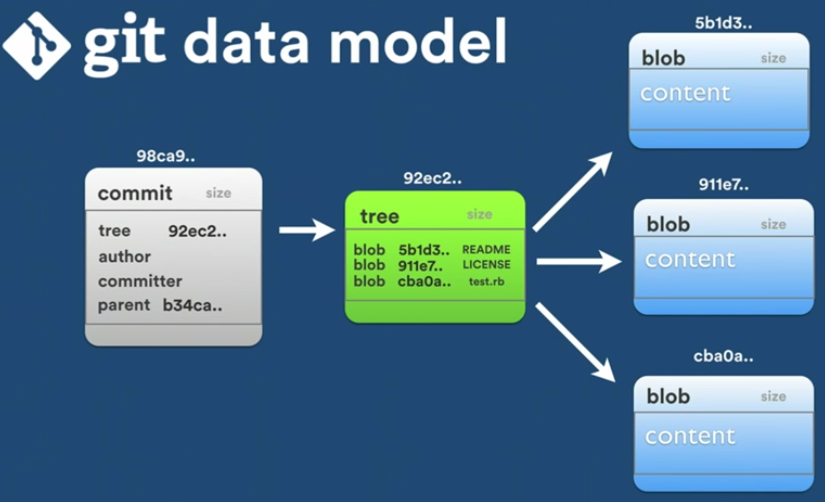
\includegraphics[width=12cm]{git_data_model.png}
  \caption{Git data model.}\label{git_data_model}
\end{figure}

Git manipulates the following objects:

\begin{itemize}
    \item[\textbullet] {commits - text files that store a description of the repository;}
    \item[\textbullet] {trees - text files that store a description of a folder;}
    \item[\textbullet] {blobs - the files that exist in your repository;}
    \item[\textbullet] {tags - text files that store information about commits.}
\end{itemize}
%
\noindent The objects are stored in the folder \emph{.git/objects}.
Each store object is identified by its SHA1 hash value, i.e. 20 bytes which identifies unequivocally the object.
The SHA1 is just an algorithm that accepts some binary information and generates 20 bytes which are ideally unique for that information. The probability of collisions is extremely low, i.e. the probability that different information generates the same hash value is extremely low.
Note that 20 bytes can be represented by a 40 characters hexadecimal string.
The identifier of each object is the 40 characters hexadecimal string.
Each particular object is stored in a sub-folder inside the \emph{.git/objects}.
The name of the sub-folder is the two most significative characters of the SHA1 hash value.
The name of the file that is inside the sub-folder is the remanning thirty eight characters of the SHA1 hash value.
The Git stores all committed versions of a file.
The Git maintains a contend-addressable file systems, i.e. a file system in which the files can be accessed based on its contend. Lets look more carefully in each stored object.

A \textbf{commit} object is identified by a SHA1 hash value, and has the following information: a pointer for a tree (the root), a pointer for the previous commit, the author, the committer and a commit message.
The author is the person who did the work. The committer is the person who validate the work and who apply the work by doing the commit. By doing this difference git allow both to get the credit, the author and the committer. Example of a commit file contend:\\
\\
tree 2c04e4bad1e2bcc0223239e65c0e6e822bba4f16\\
parent bd3c8f6fed39a601c29c5d101789aaa1dab0f3cd\\
author NetXPTO <netxpto@gmail.com> 1514997058 +0000\\
committer NetXPTO <netxpto@gmail.com> 1514997058 +0000\\
\\
Here goes the commit message.\\

A \textbf{tree} object is identified by a SHA1 hash value, and has a list of blobs and trees that are inside that tree.
A tree object identifies a folder and its contend.
Example of a tree file contend:\\
\\
\begin{tabular}{l l l l}
100644 & blob & bdb0cabc87cf50106df6e15097dff816c8c3eb34 &   .gitattributes\\
100644 & blob & 50492188dc6e12112a42de3e691246dafdad645b &   .gitignore\\
100644 & blob & 8f564c4b3e95add1a43e839de8adbfd1ceccf811 &   bfg-1.12.16.jar\\
040000 & tree & de44b36d96548240d98cb946298f94901b5f5a05 &   doc\\
040000 & tree & 8b7147dbfdc026c78fee129d9075b0f6b17893be &   garbage\\
040000 & tree & bdfcd8ef2786ee5f0f188fc04d9b2c24d00d2e92 &   include\\
040000 & tree & 040373bd71b8fe2fe08c3a154cada841b3e411fb &   lib\\
040000 & tree & 7a5fce17545e55d2faa3fc3ab36e75ed47d7bc02 &   msbuild\\
040000 & tree & b86efba0767e0fac1a23373aaf95884a47c495c5 &   mtools\\
040000 & tree & 1f981ea3a52bccf1cb00d7cb6dfdc687f33242ea &   references\\
040000 & tree & 86d462afd7485038cc916b62d7cbfc2a41e8cf47 &   sdf\\
040000 & tree & 13bfce10b78764b24c1e3dfbd0b10bc6c35f2f7b &   things\_to\_do\\
040000 & tree & 232612b8a5338ea71ab6a583d477d41f17ebae32 &  visualizerXPTO\\
040000 & tree & 1e5ee96669358032a4a960513d5f5635c7a23a90 &   work\_in\_progress\\
\end{tabular}
\\[5mm]

A \textbf{blob} is identified by a SHA1 hash value, and has the file contend compressed. A git header and tailor is added to each file and the file is compressed using the zlib library. The git header is just the object type, a space character, the file size in bytes and the \textbackslash NUL caracter, for instance "blob 13\textbackslash NUL", the tailor is just the \textbackslash n caracter. The compressed blob (header+file contend+tailer) is stored as a binary file.

There are two types of \textbf{tags}, lightweight and annotated tags. Lightweight tags are only a ref to a commit, see section below. Annotated tags are objects stored as text files, which as has information about the commit, to each the tag point, the tagger (name and e-mail), tag date and a tag message.

\subsection{Objects Folder}

Git stores the database and the associated information in a set of folders and files inside the the folder \emph{.git} in the root of your repository.

The folder \emph{.git/objects} stores information about all objects (commits, trees, blobs and annotated tags).
The objects are stored in files inside folders.
The name of the folders are the 2 first characters of the SHA1 40 characters hexadecimal string.
The name of the files are the other 38 hexadecimal characters of the SHA1.
The information is compressed to save space.

\section{Refs}

SHA1 hash values are hard to memorize by humans. To make life easier to humans we use refs. A ref associate a name, easier to memorize by humans, with a SHA1 hash value, used by the computer. Therefore refs are pointers to objects. Refs are implementes by text files, the name of the file is the name of the ref and inside the file is a string with the SHA1 hash value.
Tags and branches are example of refs. Tags are static references, i.e. tags are never updated, and branches are dynamic references, i.e. branches are always automatically updated.

\subsection{Refs Folder}

The \emph{.git/refs} folder has inside the following folders \emph{heads}, \emph{remotes}, and \emph{tags}.
The \emph{heads} has inside a ref for all local branches of your repository.
The \emph{remotes} folder has inside a set of folders with the name of all remote repositories, inside each folder is a ref for all branches in that remote repository.
The \emph{tag} folder has a ref for each tag.


\subsection{Branch}

A branch is a ref that points for a commit that is originated by a divergence from a common point.
A branch is automatically atualize so that it always points for the most recent commit of that branch.

\subsection{Heads}

Heads is a pointer for the branch where we are.
If we are in a commit that is not pointed by a branch we are in a detached HEAD situation.

\section{Git Logical Areas}

Git uses several spaces.

\begin{itemize}
    \item[\textbullet] {Working tree - is your directories where you are working;}
    \item[\textbullet] {Staging area or index - temporary area used to specify which files are going to be committed in the next commit;}
    \item[\textbullet] {History - recorded commits;}
\end{itemize}

All information related with the staging area and the history is stored in the \emph{.git} folder.

\begin{figure}[h!]
  \centering
  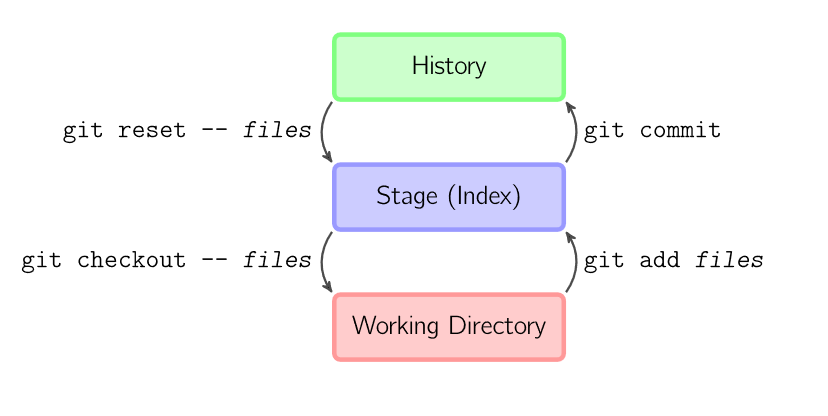
\includegraphics[width=12cm]{git_logical_areas.png}
  \caption{Git logical areas. Figure adapted from~\cite{Lodato19}.}\label{git_logical_areas}
\end{figure}

\section{Merge}

Merge is a fundamental concept to git. It is the way you consolidate your work.

\subsection{Fast-Forward Merge}

It is used when there is a direct path between the two branches, the older branch is just updated.

\subsection{Three-Way Merge}

It is used when there is no direct path between the two branches. In this case a common commit is found considering the two branches and the merge is performed using a recursive strategy.
In this process conflicts can occur.
The recursive strategy is applied to each modified file and line by line.
If the line was not modified in both branches the line is not modified in the merged file.
If the line was modified only in one branch the line is going to be modified in the merged file.
If the line is modified in both branches Git cannot make a decision and a conflict occur.
So, conflicts occur when branches that change the same file in the same line are being merged.

\section{Remotes}

A remote is a repository in another location. The remote location can be the http://github.com or the location of any other Git server.

\subsection{GitHub}

GitHub is a Git server that stores public repositories.
A GitHub user will have a user name and password and inside his or her account creates public repositories.
This repositories can be transferred to a local machine using the command \emph{git clone <repository url>}.
The local and remote repository will be linked and the local repository can be updated using the \emph{git fetch} or \emph{git pull} command.
The remote repository can be updated using the \emph{git push} command.
When the remote repository is cloned an alias, named origin, is created that points to that remote repository.
Another way to create a GitHub repository is by forking another existente repository.
Forked repositories are linked and they can be syncronized using pull requests.

\begin{figure}[h!]
  \centering
  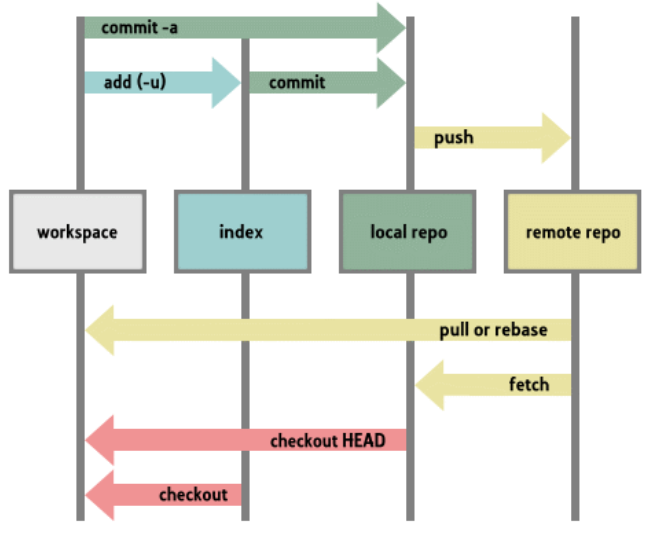
\includegraphics[width=12cm]{git_spaces.png}
  \caption{Git remotes.}\label{git_remotes}
\end{figure}

\section{Commands}


\subsection{Porcelain Commands}

Porcelain commends are high-level commands.

\vspace*{5mm} \noindent \textbf{git add}

\noindent \emph{git add}, adds a a new or modified file (or files) to the staging area.

\vspace*{5mm} \noindent \textbf{git branch}

\noindent \emph{git branch}, lists local branches.

\noindent \emph{git branch -r}, lists remote branches.

\noindent \emph{git branch -a}, lists all branches.

\noindent \emph{git branch -u <remote>/<branch>}, links the local branch in which you are in with a remote branch.

\noindent \emph{git branch --set-upstream-to=<remote>/<branch>}, longer version of the previous command.

\noindent \emph{git branch -u <remote>/<branch> <local\_branch>}, links the local branch with a remote branch.

\noindent \emph{git branch --set-upstream-to=<remote>/<branch> <local\_branch>}, longer version of the previous command.

\vspace*{5mm} \noindent \textbf{git cat-file}

\noindent \emph{git cat-file -t <hash>}, shows the type of the object identified by the hash value.

\noindent \emph{git cat-file -p <hash>}, shows the contend of the file associated with the object identified by the hash value.


\vspace*{5mm} \noindent \textbf{git checkout}

\noindent \emph{git checkout -b <new\_branch\_name>}, creates a new branch in the same position as the current branch and move to it.

\noindent \emph{git checkout -b <new\_branch\_name> <branch\_name>}, create a new branch in the position of <branch\_name> and move to it.

\vspace*{5mm} \noindent \textbf{git clean}

\noindent \emph{git clean -f -d}, removes from the working directory all untracked directories (d) and files (f).

\vspace*{5mm} \noindent \textbf{git clone}

\noindent \emph{git clone <url>}, downloads the contend of the <url> repository, for instance http://www.github.com/netxpto/linkplanner.git, and creates a local repo.

\vspace*{5mm} \noindent \textbf{git config}

\noindent \emph{git config --global user.name "netxpto"}, sets the user name globally.

\noindent \emph{git config --global user.email "netxpto.gmail.com"}, sets the user e-mail globally.

\noindent \emph{git config --global user.emmail "netxpto.gmail.com"}, sets the user e-mail globally.

\noindent \emph{git config --global alias.<alias name> <commands>}, creates a global alias for the commands.

\vspace*{5mm} \noindent \textbf{git diff}

\noindent \emph{git diff}, shows the changes between the working space and the staging area.

\noindent \emph{git diff --name-only}, shows the changes between the working space and the staging area, in the specified files.

\noindent \emph{git diff --cached}, shows the changes between the staging area and the current branch history. Note that --cached or --staged are synonymous.

\noindent \emph{git diff --cached --name-only}, shows the changes between the staging area and the current branch history, in the specified files.

\begin{figure}[H]
  \centering
  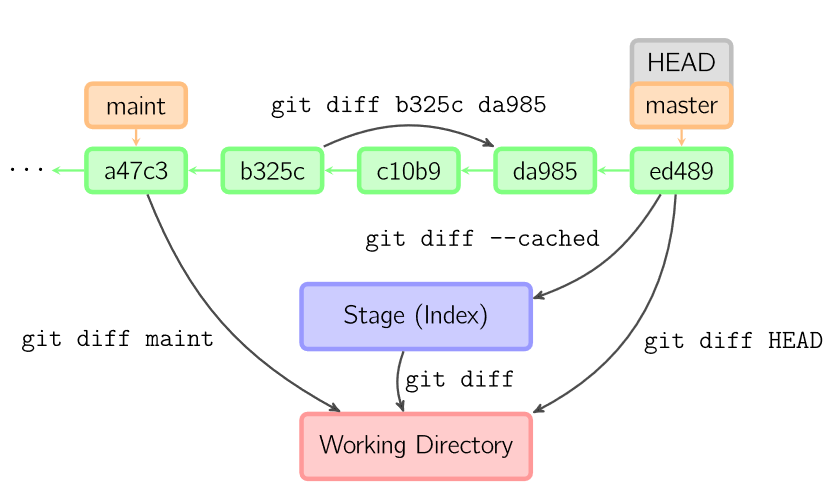
\includegraphics[width=12cm]{git_diff.png}
  \caption{Git diff command. Figure adapted from~\cite{Lodato19}.}\label{git_diff_command}
\end{figure}

\vspace*{5mm} \noindent \textbf{git fetch}

\noindent\emph{git fetch --all}, downloads all history from all remote repositories.

\noindent\emph{git fetch <repository>}, downloads all history from the remote repository.

\vspace*{5mm} \noindent \textbf{git init}

\noindent\emph{git init}, inicializes a git repository. It creates the \emph{.git} folder and all its subfolders and files.

\vspace*{5mm} \noindent \textbf{git log}

\noindent\emph{git log}, shows a list of commits from reverse time order.

\noindent\emph{git log --graph --decorate --oneline <commit1>..<commit1>}, shows the history of the repository in a colourful way.

\noindent\emph{git log --graph}, shows a graphical representation of the repository commits history.

\noindent\emph{git log --stat}, shows the name of the files that were changed in each commit

\noindent\emph{git log --follow <file>}, lists version history for a file, including rename.

\vspace*{5mm} \noindent \textbf{git ls-files}

\vspace*{5mm} \noindent \textbf{git ls-remote}

\vspace*{5mm} \noindent \textbf{git merge}

\noindent\emph{git merge <branch>}, combines the specified branch’s history into the current branch.

\vspace*{5mm} \noindent \textbf{git pull}

\noindent\emph{git pull}, downloads remote branch history and incorporates changes.

\vspace*{5mm} \noindent \textbf{git push}

\noindent\emph{git push}, uploads local branch commits to remote repository branch.

\vspace*{5mm} \noindent \textbf{git rebase}

\noindent\emph{git rebase <branch2 or commit2>}, finds a common point between the current branch and branch2 or commit2, reapply all commits of your current branch from that divergent points on top of branch2 or commit2, one by one.

\vspace*{5mm} \noindent \textbf{git remote}

\noindent\emph{git remote}, shows a list of existing remotes.

\noindent\emph{git remote -v}, shows the full location of existing remotes.

\noindent\emph{git remote add <remote name> <remote repository url>}, adds a remote.

\noindent\emph{git remote remove <remote name>}, removes a remote.

\vspace*{5mm} \noindent \textbf{git reset}

\noindent\emph{git reset --soft <commit\_hash\_value>}, moves to the commit identified by <commit\_hash\_value> but leaves in the staging area all modified files.

\noindent\emph{git reset --hard <commit\_hash\_value>}, moves to the commit identified by <commit\_hash\_value> and cleans all modified tracked files.

\noindent\emph{git reset <commit\_hash\_value>}, this is a mix reset (is the default reset), puts all modified files in the working area.

\noindent\emph{git reset <file>}, unstages the file, but preserve its contents.

\vspace*{5mm} \noindent \textbf{git reflog}

\noindent\emph{git reflog}, shows all commands from the last 90 days. Git only perform garbaged collection after 30 days.

\vspace*{5mm} \noindent \textbf{git rm}

\noindent\emph{git rm <file>}, deletes the file from the working directory and stages the deletion.

\noindent\emph{git rm --cached <file>}, removes the file from version control but preserves the file locally.

\vspace*{5mm} \noindent \textbf{git show}

\noindent\emph{git show}, shows what is new in the last commit.

\vspace*{5mm} \noindent  \textbf{git stash}

\noindent\emph{git stash}, temporarily stores all modified tracked files.

\noindent\emph{git stash --list}, shows what is in the stash.

\noindent\emph{git stash pop}, restores the most recently stashed files.

\noindent\emph{git stash drop}, discards the most recently stashed changeset.

\vspace*{5mm} \noindent \textbf{git status}

\noindent\emph{git status}, lists all new or modified files to be committed.

\subsection{Pluming Commands}

Pluming commands are low-level commands.

\vspace*{5mm} \noindent \textbf{git cat-files}

\noindent \emph{git cat-files -p <sha1>}, shows the contend of a file in a pretty (-p) readable format.

\noindent \emph{git cat-files -t <sha1>}, shows the type of a object, i.e. blob, tree or commit.

\vspace*{5mm} \noindent \textbf{git count-object}

\noindent \emph{git count-object -H}, counts all object and shows the result in a (-H) human readable form.

\vspace*{5mm} \noindent \textbf{git gc}

\noindent \emph{git gc}, garbage collector, eliminates all objects that has no reference associated with.

\noindent \emph{git gc --prune=all}


\vspace*{5mm} \noindent \textbf{git hash-object}

\noindent \emph{git hash-object <file>}, calculates the SHA1 hash value of a file plus a header.

\noindent \emph{git hash-object -w <file>}, calculates the SHA1 hash value of a file plus a header and write it in the \emph{.git/objects} folder.

\vspace*{5mm} \noindent \textbf{git merge-base}

\noindent \emph{git merge-base <branch1> <brach2>}, finds the base commit for the three-way merge between <branch1> and <branch2>.


\vspace*{5mm} \noindent \textbf{git update-index}

\noindent \emph{git update-index --add <file name>}, creates the hash and adds the <file\_name> to the index.

\vspace*{5mm} \noindent \textbf{git ls-files}

\noindent \emph{git ls-files --stage}, shows all files that you are tracking.

\vspace*{5mm} \noindent \textbf{git write-tree}

\vspace*{5mm} \noindent \textbf{git commit-tree}

\vspace*{5mm} \vspace*{5mm} \noindent \textbf{git rev-parse}

\noindent \emph{git rev-parse <ref>}, return the hash value of <ref>.

\noindent \emph{git rev-parse <short\_hash\_value>}, return the full hash value associated with <short\_hash\_value>.


\vspace*{5mm} \noindent \textbf{git update-ref}

\noindent \emph{git update-ref refs/heads/<branch name> <commit sha1 value>}, creates a branch that points to the <commit sha1 value>.

\vspace*{5mm} \noindent \textbf{git verify-pack}

\section{Navigation Helpers}

\noindent \emph{<ref>$^{\wedge}$}, one commit before <ref>.

\noindent \emph{<ref>$^{\wedge \wedge}$}, two commits before <ref>.

\noindent \emph{<ref>$\sim$5}, five commits before <ref>.

\noindent \emph{<ref1>..<ref2>}, between commit <ref1> and <ref2>.

\noindent \emph{<branch>$^{\wedge}${tree}}, identifies the tree pointed by the commit pointed by <branch>.

\noindent \emph{<commit>:<file\_name>}, identifies the version of a file in a given commit.

\section{Configuration Files}

There is a config file for each repository that is stored in the \emph{.git/} folder with the name \emph{config}.\\
\\
There is a config file for each user that is stored in the \emph{c:/users/<user name>/} folder with the name \emph{.gitconfig}.\\
\\
To open the \emph{c:/users/<user name>/.gitconfig} file type:\\
\\
\textbf{git config --global -e}

\section{Pack Files}

Pack files are binary files that git uses to save data and compress your repository. Pack files are generated periodically by git or with the use of gc command.

\section{Applications}

\subsection{Meld}

%# --------------------------------------D I F F -----------------------------
%
%[diff]
%    guitool = meld
%
%[difftool "meld"]
%    cmd = \"C:/Program Files (x86)/Meld/Meld.exe\" \"$LOCAL\" \"$REMOTE\" --label \"DIFF (ORIGINAL MY)\"
%	
%# --------------------------------------M E R G E -----------------------------
%
%[merge]
%    tool = meld
%
%[mergetool "meld"]
%    cmd = \"C:/Program Files (x86)/Meld/Meld.exe\" --auto-merge \"$LOCAL\" \"$BASE\" \"$REMOTE\" --output \"$MERGED\" --label \"MERGE (REMOTE BASE MY)\"
%    trustExitCode = false
%
%[mergetool]
%    # don't ask if we want to skip merge
%    prompt = false
%
%    # don't create backup *.orig files
%    keepBackup = false

\subsection{GitKraken}

\section{Error Messages}

\subsection{Large files detected}

Clean the repository with the \href{https://rtyley.github.io/bfg-repo-cleaner}{BFG Repo-Cleaner}.\\
\\
Run the Java program:\\

java -jar bfg-1.12.16.jar \texttt{-{}-}strip-blobs-bigger-than 100M\\
\\
This program is going to remote from your repository all files larger than 100MBytes. After do:\\

git push \texttt{-{}-}force.

\section{Git with Overleaf}

You can use git with overleaf.
For that you have to create a project on overleaf.
Associate with that overleaf project it is also create a git repository.
The address of that git repository is almost the same as the overleaf project that you can obtain going to the overleaf Menu/Share. Let's assume that the overleaf project address is:\\
\\
\noindent https://www.overleaf.com/12925162jkwbhrdkwrfm\\
\\
In this case the repository address is https://git.overleaf.com/12925162jkwbhrdkwrfm\\
%
The only change was the replacement of \textbf{www} by \textbf{git}.

Now you can just do

git clone https://git.overleaf.com/12925162jkwbhrdkwrfm

and clone your repository.

You can also do

git push https://git.overleaf.com/12925162jkwbhrdkwrfm


% bibliographic references for the section ----------------------------
\clearpage
\printbibliography[heading=bibliography]
\end{refsection}
\addcontentsline{toc}{section}{Bibliography}
\cleardoublepage
% ---------------------------------------------------------------------

